\documentclass{beamer}
\usepackage[utf8]{inputenc}
\usepackage{amsmath, pdfpages, pdflscape, lscape, color, listings, hyperref, amssymb, graphicx,textcomp,varioref, afterpage, subcaption, float, bm, tikz, multicol} 

\global
\newcommand{\Fig}[1]{Figure \ref{#1}}
\newcommand{\fig}[1]{figure \ref{#1}}
\newcommand{\tab}[1]{table \ref{#1}}
\newcommand{\eq}[1]{equation \ref{#1}}
\newcommand{\Eq}[1]{Equation \ref{#1}}
\newcommand{\alg}[1]{algorithm \ref{#1}}
\newcommand{\Alg}[1]{Algorithm \ref{#1}}
\newcommand{\chp}[1]{chapter  \ref{#1}}
\newcommand{\Chp}[1]{Chapter  \ref{#1}}
\newcommand{\e}[1]{\cdot 10^{#1}}
\newcommand{\h}{\hbar}
\newcommand{\der}[2]{\frac{\partial #1}{\partial #2}}
\newcommand{\dder}[2]{\frac{\partial^2 #1}{\partial #2^2}}
\newcommand{\p}{\boldsymbol{P}}
\newcommand{\q}{\boldsymbol{q}}
\newcommand{\norm}[1]{\left\lVert#1\right\rVert}
\newcommand{\coef}[2]{\frac{\langle #1,#2\rangle_Q}{\norm{#2}^}}


\DeclareMathOperator*{\argmin}{argmin}
\DeclareMathOperator*{\argmax}{argmax}

\newcommand{\E}[1]{\mbox{E}\!\left(#1\right)}
\newcommand{\Var}[1]{\mbox{Var}\!\left(#1\right)}
\newcommand{\Cov}[1]{\mbox{Cov}\!\left(#1\right)}

\newenvironment{test}[1]
{
 \usebackgroundtemplate{}
 \color{gray!30!black}
   \begin{tikzpicture}[remember picture, overlay]
     \node[anchor = center, opacity=.25] (image) at (current page.center) {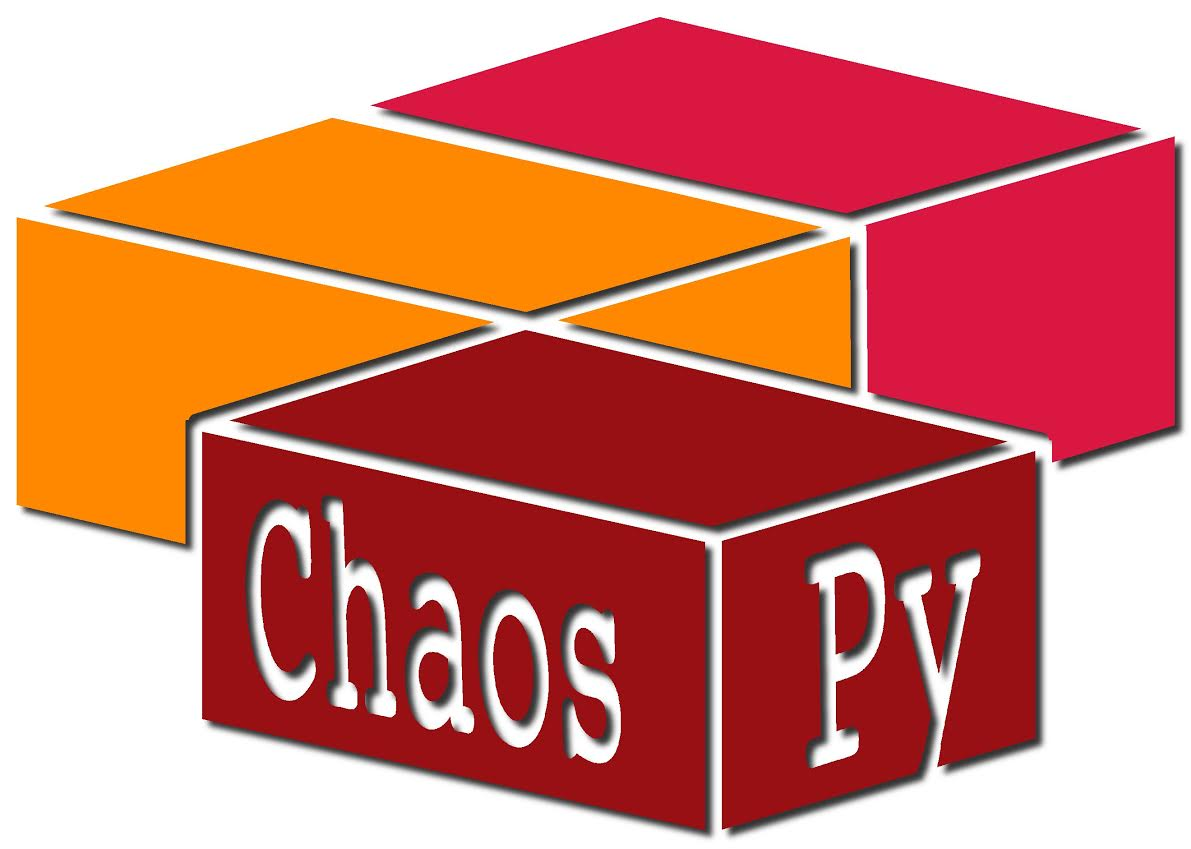
\includegraphics[scale=0.25]{chaospy_logo.jpg}};
   \end{tikzpicture}
 \begin{frame}[fragile,enviroment=chaospy]
   
}
{
 \end{frame}
}

\lstset{
escapeinside=||
}


\newenvironment{chaospy}[1]
{\color{gray!30!black}
     \color{gray!30!black}
     \usebackgroundtemplate{
   \begin{tikzpicture}[remember picture, overlay]
     \node[anchor = center, opacity=.25] (image) at (current page.center) {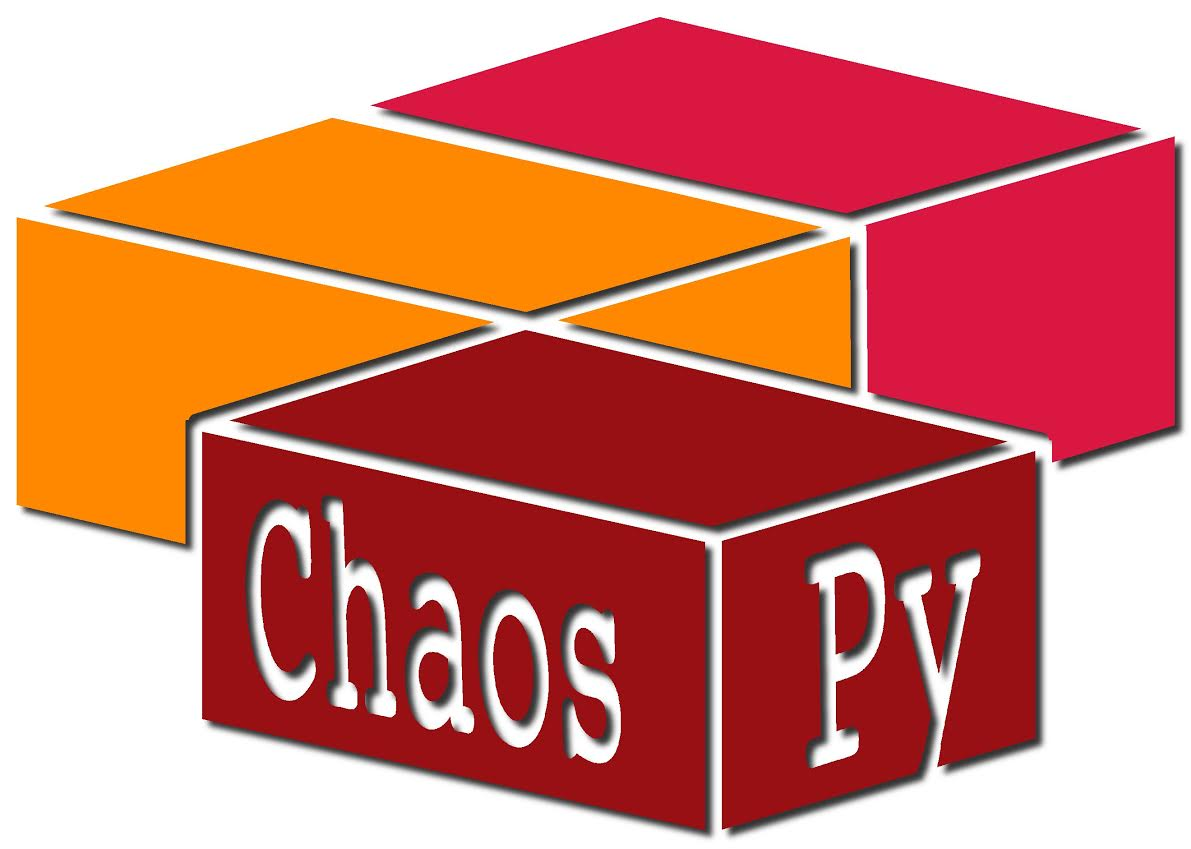
\includegraphics[scale=0.25]{chaospy_logo.jpg}};
   \end{tikzpicture}}
     \begin{frame}[fragile,environment=chaospy]
    \frametitle{{#1}}}
{\end{frame}}


\definecolor{keywords}{RGB}{255,0,90}
\definecolor{comments}{RGB}{0,0,113}
\definecolor{red}{RGB}{160,0,0}
\definecolor{green}{RGB}{0,150,0}
 
\usetheme{kalkulo}

\graphicspath{{./figures/}}


\title{Polynomial chaos expansions part 3: Advanced topics - Dependent variables}
\author{Jonathan Feinberg and Simen Tennøe}


\begin{document}



\begin{frame}
  \maketitle
\end{frame}


\begin{frame}
 \frametitle{Dependence}
 \begin{figure}
 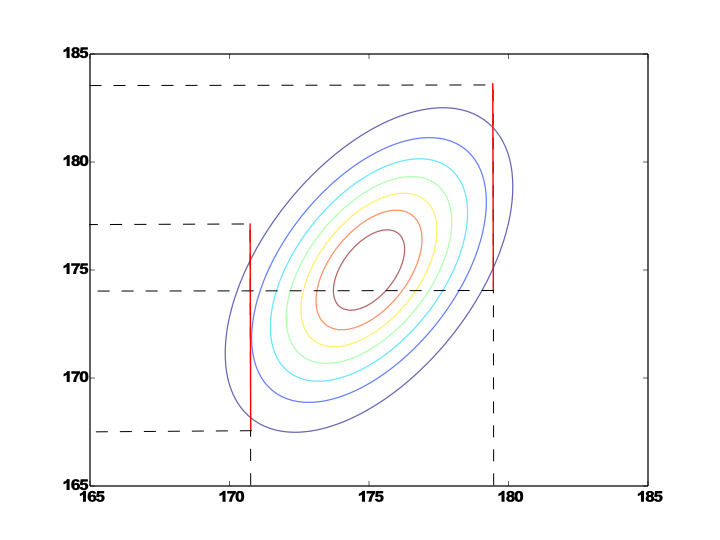
\includegraphics[width = 0.9\textwidth]{dependent.png}
 \end{figure}

 \end{frame}

 
 \begin{chaospy}{Repetition: Full 2D implementation}
     \scriptsize
 \begin{lstlisting}[language=python]
def u(x,a, I):
  return I*np.exp(-a*x)
|\pause|
a = cp.Uniform(0, 0.1)
I = cp.Uniform(8, 10)
dist = cp.J(a,I)|\pause|
|\pause|
P = cp.orth_ttr(2, dist)
|\pause|
nodes, weights = \
    cp.generate_quadrature(3, dist, rule="G")
|\pause|
x = np.linspace(0, 10, 100)
solves = [u(x, *node) for node in nodes.T]
|\pause|
u_hat = cp.fit_quadrature(P, nodes, weights, solves)
|\pause|
mean, var = cp.E(u_hat, dist), cp.Var(u_hat, dist)
 \end{lstlisting}
\end{chaospy}
 

\begin{frame}
 \frametitle{Dependent variables}
 % TODO
 % copy code from lecture1
 \[  P_{\mathfrak i} = P_{i_1}^{(1)}P_{i_2}^{(2)}\cdots P_{i_D}^{(D)} \qquad \mathfrak i = (i_1,i_2,...,i_D)\]
 \pause
 \begin{align*}
  \langle P_\mathfrak{i},P_\mathfrak{j}\rangle &= E(P_\mathfrak{i},P_\mathfrak{j})\\
  \onslide<3-> {&=\E{P_{i_1}^{(1)}\cdots P_{i_D}^{(D)}P_{j_1}^{(1)}\cdots P_{j_D}^{(D)}}}\\ 
  \onslide<4-> {&=\E{P_{i_1}^{(1)}P_{j_1}^{(1)}}\cdots \E{P_{i_D}^{(D)}P_{j_D}^{(D)}}}\\ 
  \onslide<5-> {&=\langle P_{i_1}^{(1)}P_{j_1}^{(1)}\rangle\cdots \langle P_{i_D}^{(D)}P_{j_D}^{(D)}\rangle}\\ 
  \onslide<6-> {&=\norm{P_{i_1}^{(1)}}^2\delta_{i_1j_1}\cdots \norm{P_{i_D}^{(D)}}^2\delta_{i_Dj_D}}\\ 
  \onslide<7-> { \langle P_\mathfrak{i},P_\mathfrak{j}\rangle &=\norm{P_{\mathfrak{i}}^{(1)}}\delta_{\mathfrak{i}\mathfrak{j}}}
 \end{align*}
 \onslide<7->
\begin{alert}{But the problem is:}
\[\E{uv} \neq \E{u}\E{v} \qquad \text{when $u$ and $v$ are dependent}\]
 \end{alert}

\end{frame}



 
 
\begin{chaospy}{Simple transformation code}
 \scriptsize
 \begin{lstlisting}[language=Python]
x = np.linspace(0, 1, 100)
def u(x,a, I):
  return I*np.exp(-a*x)

C = [[2,1],[1,2]]
mu = [0.5,0.5]
|\pause|
R = cp.J(cp.Normal(),cp.Normal())
|\pause|
L =  np.linalg.cholesky(C)      # C = np.dot(L.T, L)
|\pause|
def T(r):
    return np.dot(L,r) + mu
|\pause|
P = cp.orth_ttr(M, R)|\pause|
nodes0, weights = cp.generate_quadrature(M+1, R, rule="G")|\pause|
nodes1 = T(nodes0)
|\pause|
solves = [u(x, *node) for node in nodes1.T]
|\pause|
U_analytic = cp.fit_quadrature(P, nodes0, weights, solves)
\end{lstlisting}
\end{chaospy}

\begin{frame}
 \frametitle{Convergence of transformation}
 % TODO
 % Extend to the right
 \begin{figure}
 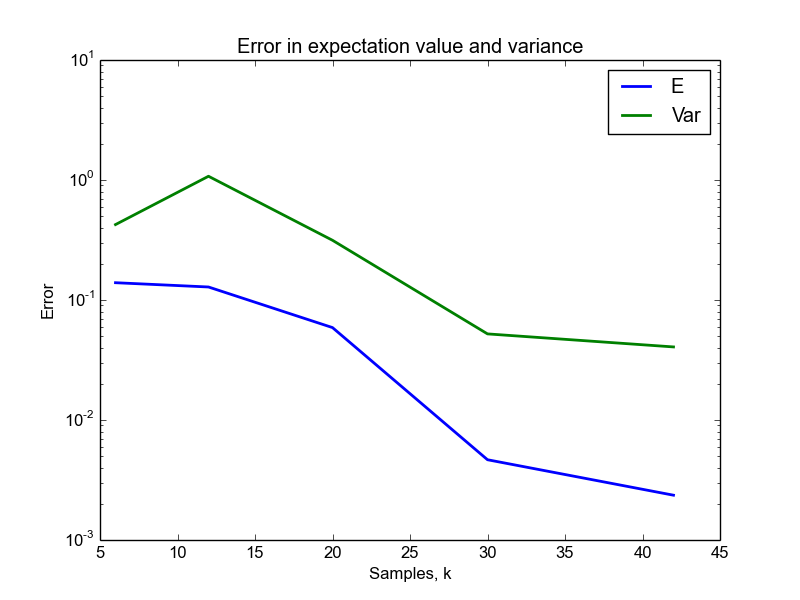
\includegraphics[width = 0.85\textwidth]{convergence_dependence.png}
 \end{figure}
 \end{frame}


 % TODO
 % use contourf
 \begin{frame}
 \frametitle{Rosenblatt Transformations}
 \begin{figure}
 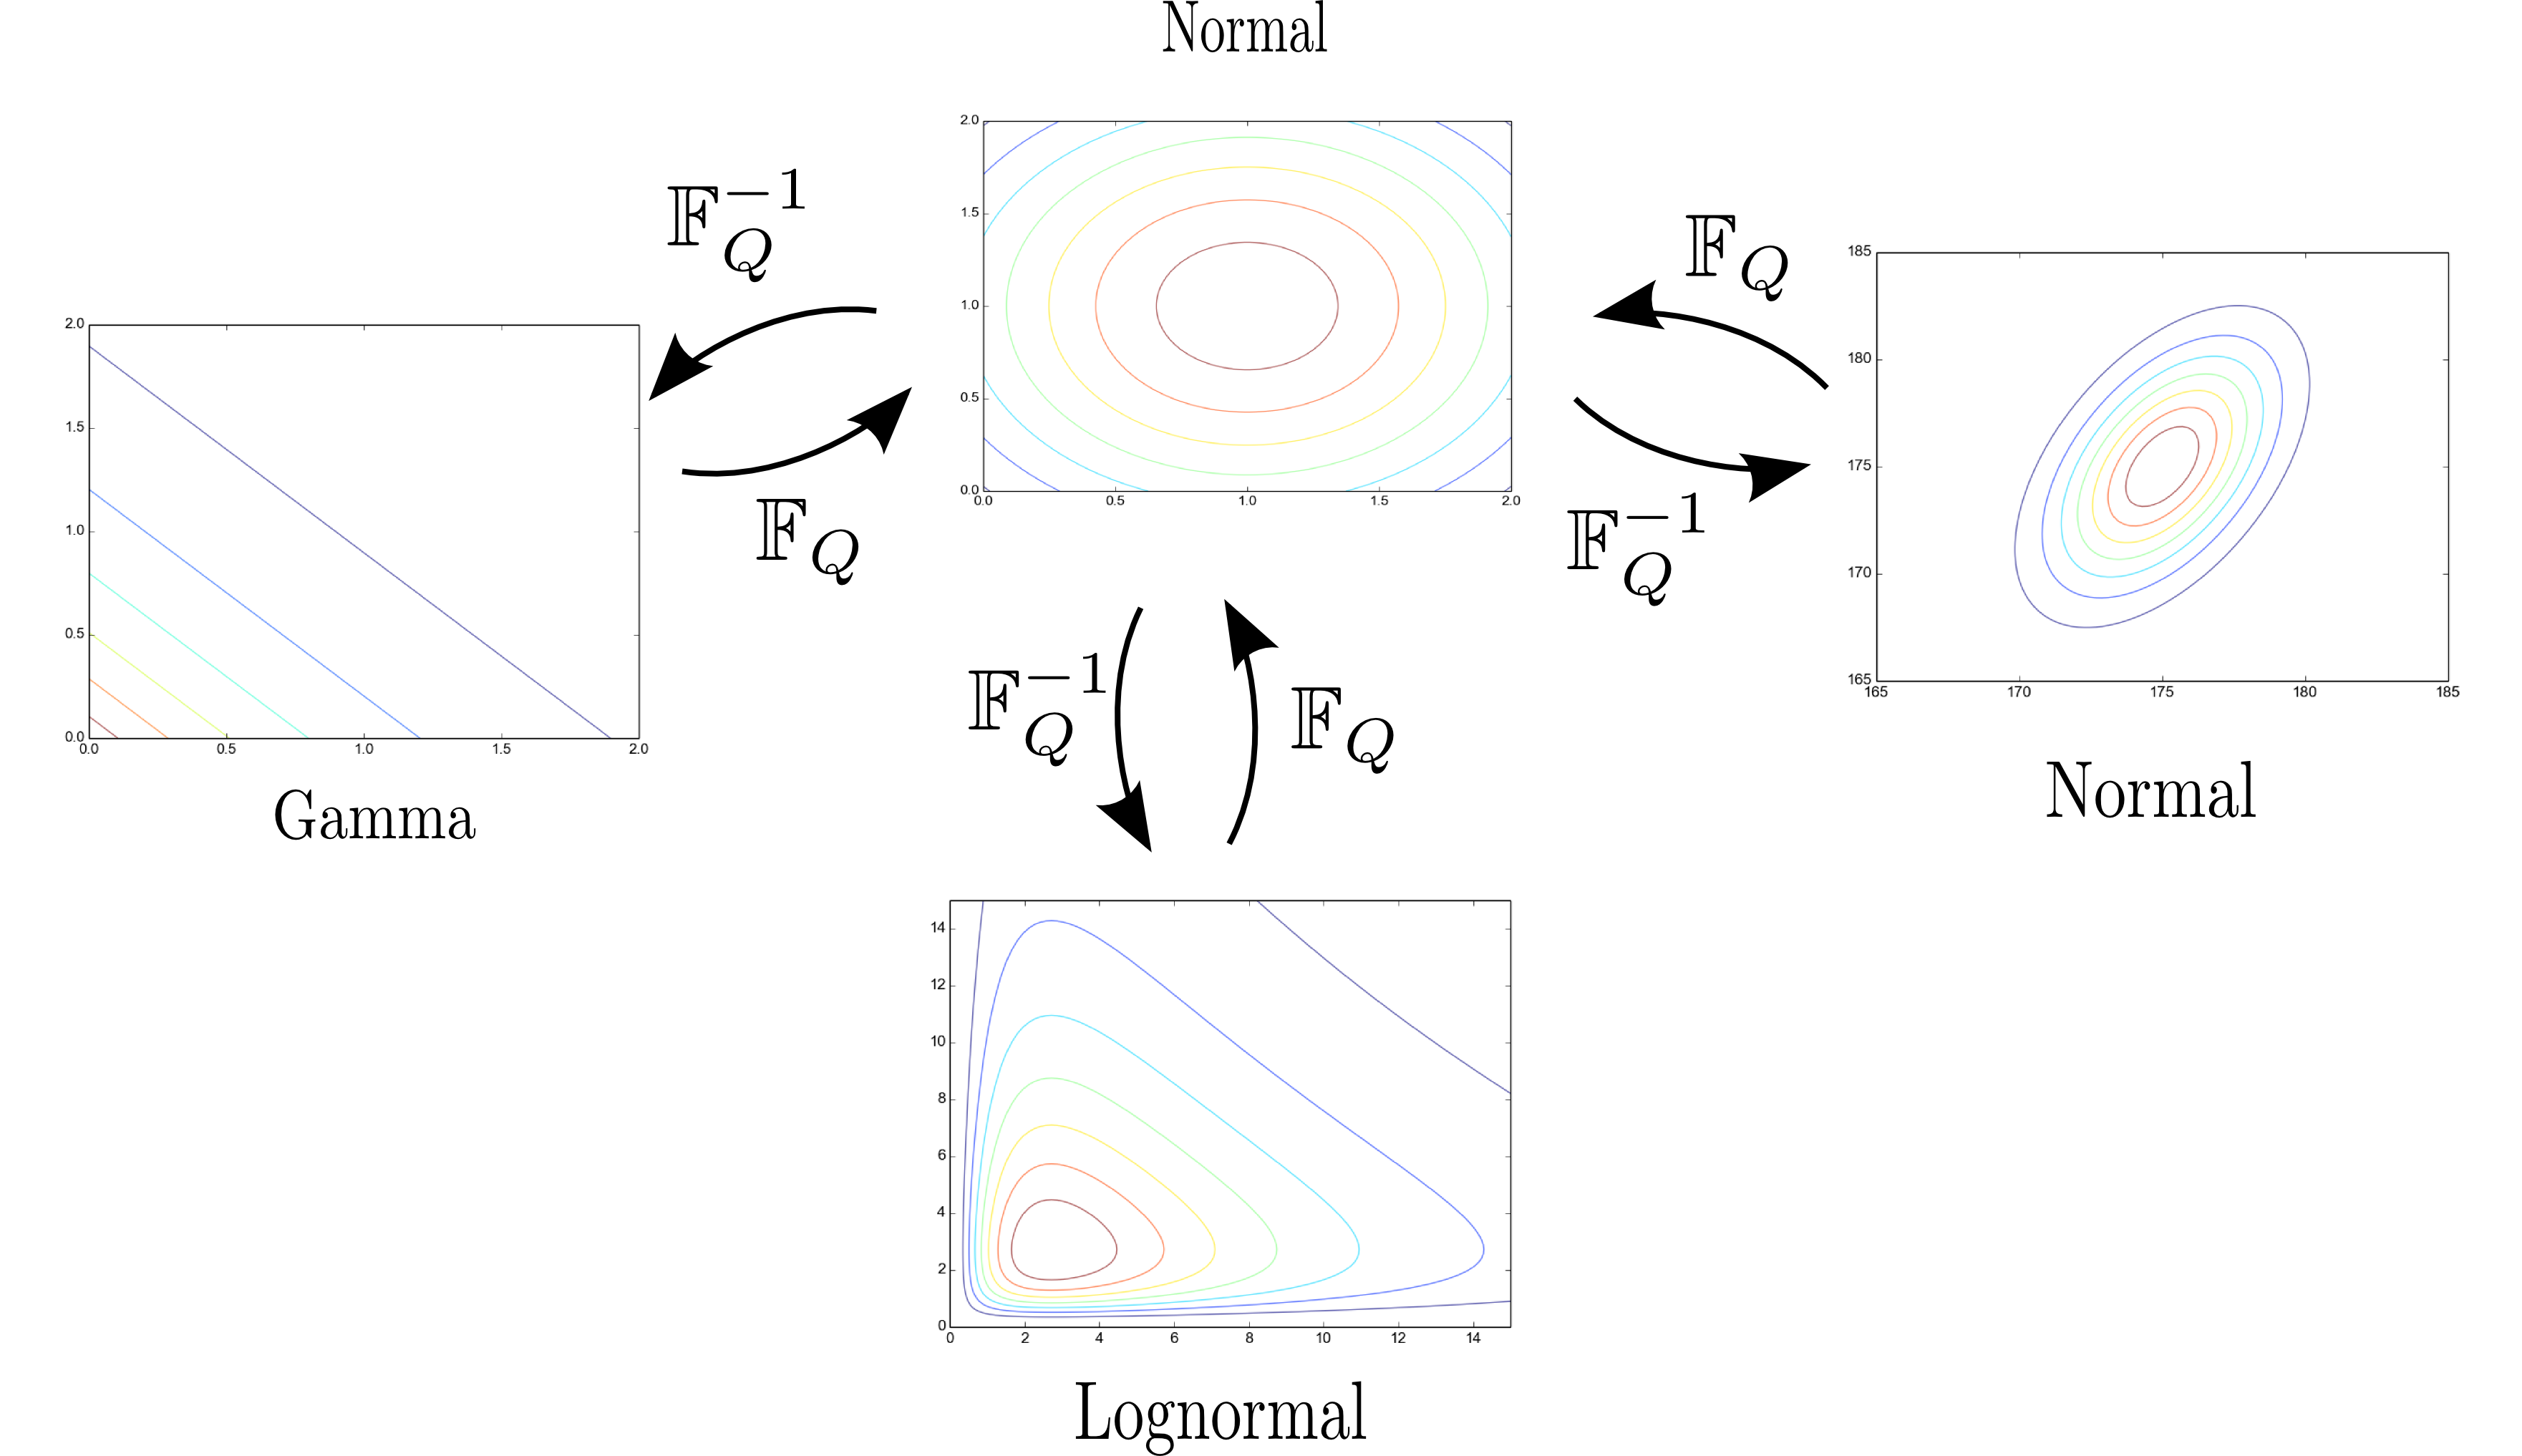
\includegraphics[width = \textwidth]{distributions.png}
 \end{figure}

 \end{frame}
 
 
 \begin{chaospy}{Rosenblatt transformation, code}
 \scriptsize
 \begin{lstlisting}[language=Python]
def u(x,a, I):
    return I*np.exp(-a*x)
|\pause|
C = [[2,1],[1,2]]
mu = np.array([0.5,0.5])
dist_R = cp.J(cp.Normal(),cp.Normal())
dist_Q = cp.MvNormal(mu,C)
|\pause|
x = np.linspace(0, 1, 100)
dt = x[1]-x[0]
M = 5

P = cp.orth_ttr(M, dist_R)|\pause|
s_R = dist_R.sample(2*len(P), "M")|\pause|
s_Q = dist_Q.inv(dist_R.fwd(s_R))|\pause|

solves = [u(x, s[0], s[1]) for s in s_Q.T]|\pause|
U_hat = cp.fit_regression(P, s_R, solves,rule="LS")
\end{lstlisting}
\end{chaospy}

 \begin{frame}
 \frametitle{Convergence of Rosenblatt transformations}
 % TODO
 % fix legend
 \begin{figure}
 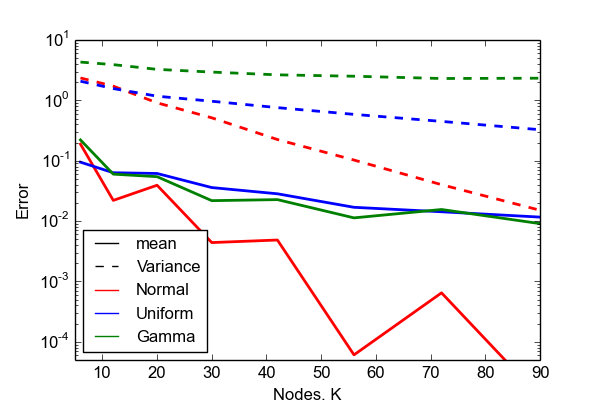
\includegraphics[width = 0.9\textwidth]{rosenblatt.png}
 \end{figure}

 \end{frame}
  

\end{document}
